\documentclass{article}
\usepackage[T1]{fontenc}
\usepackage{lmodern}
\usepackage{graphicx}
\usepackage{amsmath,amssymb}
\usepackage[a4paper,margin=2cm]{geometry}
\usepackage[absolute,overlay]{textpos}
\setlength{\TPHorizModule}{1mm}
\setlength{\TPVertModule}{1mm}
\usepackage[indonesian]{babel}
\usepackage{hyperref}
\setlength{\emergencystretch}{2em}
% unit: Halaman 10

\begin{document}

% === Halaman 10 (python/native) ===

Penjumlahan Titik pada Kurva Eliptik

(a) P + Q = R

10

Penjelasan geometri:

1.

Tarik garis melalui P dan Q

2.

Jika P  Q, garis tersebut 


memotong kurva pada titik  -R

3.     Pencerminan titik -R terhadap


sumbu-x adalah titik R

4.

Titik R adalah hasil 


penjumlahan titik P dan Q


Keterangan:  Jika R =(x, y) maka –R 



        adalah titik (x, -y)

Sumber gambar: Andreas Steffen, Elliptic Curve Cryptography

% deskripsi: gambar native xref 58
\noindent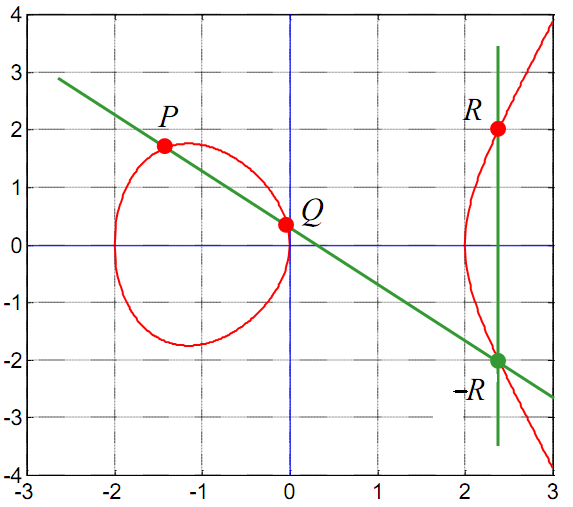
\includegraphics[width=0.85\textwidth]{../../images/python/page_010_img_01.png}

\end{document}
